\documentclass[conference]{IEEEtran}
\usepackage{ctex}
% CJK 主字体：ctex 默认字集 FandolSong 缺「濙」(U+6FD9) 等字形（PDF 会出现空白/方框），
% 必须用系统华文宋体 STSong（普通 TrueType，xdvipdfmx 可正常子集嵌入）。
% ⚠️ 不要用 Noto Serif SC：本机那版是可变字体 VF，会被 xdvipdfmx 以 Invalid TTC index 拒收。
\setCJKmainfont{STSong}
\usepackage{amsmath}
\usepackage{amssymb}
\usepackage{graphicx}
\usepackage{makecell}
\usepackage{booktabs}
\usepackage{tabulary}

% math_commands.tex —— 全文数学符号与缩略语统一定义（各篇可按需增删，勿改已有通用宏）
\newcommand{\kg}{知识图谱}
\newcommand{\corpus}{语料}
\newcommand{\salience}{叙事热度}
\newcommand{\centre}{中心性}
\newcommand{\Deg}{d}
\newcommand{\Chap}{h}
\newcommand{\Rho}{\rho}
\newcommand{\NP}{\emph{N}}
\newcommand{\bk}[1]{\textbf{#1}}
\newcommand{\cited}[1]{[\cite{#1}]}
\newcommand{\pct}[1]{#1\%}

% latex_includes.tex —— 只声明图片搜索路径与统一宽度宏
% ⚠️ 禁止在本文件里写 \begin{comment}...\end{comment} 包裹的示例 figure：
%    comment 环境需要 \usepackage{comment}，否则编译直接报
%    "LaTeX Error: Environment comment undefined"（试点篇踩过）。
% 所有 figure 环境一律写在 sections/5_results.tex 内，图题只进 \caption，图内不写标题。
\graphicspath{{figures/}}
\newcommand{\figpath}[1]{figures/#1}


% ⚠️ IEEEtran conference 类不定义参考文献栏头那个宏（那是 book/article 类的名字），
%    在本类里重定义它会使文档类报错并直接编译失败。此处沿用 conference 版式自带的英文 References 栏头。

\title{心学与朝廷：思想的突围与权力的收编\\[2pt]
\large Mind Learning and the Court: Intellectual Diffusion and Political Incorporation}

\author{Anonymous}
\date{}

\begin{document}
\maketitle

%% 中文摘要（200–350 字）：目的 → 数据 → 方法 → 三个结果（带数字）→ 首要限制
\noindent\textbf{摘要（中文）}：本文以一部民间明史通俗叙事（156章）及其结构化知识图谱为语料，检验阳明心学在该叙事中的传播是否独立于朝廷权力结构。语料含1231位人物、1106件事件与2324条关系。逐字检索显示，书中“王阳明”零命中而“王守仁”命中538次，且“致良知”仅2次、“知行合一”12次，思想语汇呈标签化层级分布。关系网络分析表明，10名思想相关人物的90条显式关系中师生同门占30.0\%，高于全图2.7\%的基线，也高于权力参照组的11.7\%；但同一批人物中权力类关系仍占58.9\%，说明师承通道是嵌入而非悬浮于权力网络。时间上，8件思想事件中5件（62.5\%）集中于1508--1528年，1579年与1593年的书院事件在结构化编码中被判为政治斗争。结论是：思想突围只在叙事修辞层面成立，其制度性收编表现为可测量的类别迁移。首要限制是语料同源，图谱编码与叙事出自同一作者，统计相关不能排除主观抽取选择。

\noindent\textbf{关键词}：阳明心学；师承网络；书院；知识图谱；数字人文；明代思想史

\vspace{6pt}
%% 英文摘要 150–250 词（aris 硬要求，不许超）
\begin{abstract}
We test whether the diffusion of Wang Yangming's moral learning in a popular Ming-history narrative is independent of court politics. The corpus comprises 156 chapters together with a structured knowledge graph of 1,231 persons, 1,106 events and 2,324 relations. Verbatim search shows that the phrase used for the philosopher is not the one modern scholarship prefers: ``Wang Yangming'' occurs zero times while ``Wang Shouren'' occurs 538 times, and the programmatic terms ``innate knowing'' and ``unity of knowledge and action'' appear only twice and twelve times respectively. Relation analysis of ten intellectually salient persons gives 90 explicit edges, of which 30.0\% are master--disciple ties, well above the whole-graph baseline of 2.7\% and above an 11.7\% power-relation control group; yet within the same persons power relations still account for 58.9\%. Mentorship therefore penetrates the power network rather than floating outside it. Temporally, five of eight intellectually tagged events (62.5\%) fall in 1508--1528, and the two late academy events of 1579 and 1593 are coded as political conflict. The narrative thus dramatizes intellectual emancipation while its encoded structure records institutional incorporation. The principal validity threat is that graph and narrative share a single source of authorship.
\end{abstract}

\begin{IEEEkeywords}
mind learning, Wang Yangming, relation network, academies, digital humanities, Ming intellectual history
\end{IEEEkeywords}

\section{引言}

万历七年，张居正下令关闭天下书院六十四处；十四年后，顾宪成被罢，东林书院的讲学又进入政治斗争叙事。若只把前者叫作“收编”、后者叫作“突围”，论文仍停在漂亮的标签上。真正可检验的问题是：思想人物在关系网络中依靠何种边扩散，又通过何种边进入朝廷冲突？思想事件在时间上是连续积累，还是在少数节点被叙事压缩？

本文把《明朝那些事儿》这一通俗史著抽取成的知识图谱作为研究对象。我们不从哲学命题真伪出发，而从叙事怎样组织人物、事件与关系出发。原文检索仅用于确认语汇确实出现；关系类别构成衡量思想传播与权力交涉的结构位置；带年份事件则给出时间序列。三类证据各自回答“说过什么”“连到谁”“何时发生”，避免用一个含混的“思想影响力”代替全部现象。

本文贡献有三点。第一，提出可复算的操作化方案：以“师生同门”作为传播替代量，以君臣从属、政治攻讦、敌对冲突、同盟友党四类边作为权力接合替代量，并把自动推导的同事件边单独剔除。第二，给出思想型人物与权力型人物的可比构成：10名思想相关人物的显式关系中，师生同门占30.0\%，权力关系占58.9\%；张居正与严嵩两名参照人物的相应比例为11.7\%与80.5\%。第三，把思想相关事件排成年表，识别1508至1528年的形成—传授密集段，以及1579和1593年的制度性冲突节点。

本文的结论有明确边界。“突围/收编”是解释框架，不是图谱字段；关系类别与年份序列只能作为替代量。语料是通俗叙事而非《传习录》、奏疏或书院档案，因而本文能够说明这部书怎样叙述心学与朝廷，不能据此复原明代思想的全部内涵，也不能把词频当作社会影响力。

\section{相关工作}

本文位于思想史、政治思想、历史网络分析与大规模文本研究四条文献脉络的交叉处。它不以图谱替代思想史，而是追问一种通俗叙事把思想写成哪些人物关系与政治节点。

\subsection{良知、德性与行动}

王阳明研究首先处理“良知”作为道德知识的性质。Huang 将良知解释为一种新儒家智慧概念，强调道德判断不是外加规则，而是主体可发动的知识\cite{huang2006}；Tien 则从道德形上学与信念正当化两端讨论王阳明，指出情感、认识与道德实践不能被拆成互不相干的层次\cite{tien2004,tien2010}。这些研究面对的是哲学论证本身，材料来自思想文本及其概念脉络。本文面对的材料不同：通俗叙事把“良知”压缩成人物语言、师承与行动场景。因此，我们不判定其阐释是否穷尽原义，只测量概念在叙事中的出现及其所连接的社会关系。

\subsection{知行关系与政治秩序}

把心学理解为行动伦理，是第二条脉络。Angle 以德性伦理学讨论王阳明，把修养、判断与行动放进同一人格结构\cite{angle2010}；Yao 通过与 Bacon 的比较，强调学习并非知识囤积，而须在行动中完成\cite{yao2013}。与此同时，Kim 对王阳明与湛若水的争论表明，新儒家并不只讨论内在修养，也触及政治统一与秩序构造\cite{kim2012}。这组文献提醒我们，不能把“思想”预设为朝廷之外的纯观念空间。本文因此把王守仁的师生同门边与君臣、攻讦、冲突、同盟边放在同一分母内观察，而不是先把他归入“思想家”后便删去政治关系。

\subsection{中心性与历史关系网络}

网络分析提供了第三条方法线索。Freeman 对中心性概念的澄清表明，度数只刻画直接连接数量，不能自动等同于权力、声望或因果影响\cite{freeman1978}。Lemercier 进一步说明，历史网络方法的价值在于把关系选择、时间边界与资料缺失公开，而非让可视化图形替历史学家代言\cite{lemercier2015}。本文遵守这一限制：度数50只说明王守仁在2324条抽取关系中的直接连接数，不等同于“思想影响力50”；类别占比说明边如何被编码，也不证明行为动机。

\subsection{远读与可回到原文的核验}

大规模语料研究展示了从文本集合中提取趋势的可能性\cite{michel2011}，但单部著作的高频词尤其容易被误读。词频会把书名、章标题、引语与作者评论一并计数；同一名字的反复出现也可能来自情节密度，而非历史重要性。本文采用“两步远读”：先用逐字检索确认“心学”“知行合一”“讲学”“书院”等词的非零命中，再回到结构化事件和关系边。文本命中是存在性证据，图谱统计是结构证据，两者不互相冒充。

\subsection{本文的位置}

既有哲学研究解释王阳明思想“是什么”，网络研究解释关系量“如何算”，远读研究解释文本模式“怎样抽取”。本文把三者收束到一个较窄的问题：一部通俗明史怎样把思想传播写成师承，又怎样把同一批人物写入朝廷权力关系。研究对象不是完整明代思想世界，而是该书可观察、可复算的叙事结构；语料版本记为无 DOI 的书籍材料\cite{dangnian2009}。

\section{语料与数据}

\subsection{语料边界}

语料为《明朝那些事儿》全七部文本，共156章。项目从文本中整理1231个人物、563个地点、1106件事件与2324条关系。原始文本受版权约束，不随论文公开；统计底稿只保存汇总值、结构化条目与命中次数。这里的“明代思想史”始终带有语料限定：它是该书选择、复述和评论过的思想史片段。

\subsection{三层观察单位}

第一层是逐字语汇。我们调用统一接口对11个候选词做完全匹配，0命中词不进入论证。保留项中，“王守仁”命中538次，“心学”38次，“理学”29次，“书院”20次，“讲学”17次，“知行合一”12次，“致良知”2次。次数是字符串出现数，不是概念段落数。

第二层是关系。全图有12类关系，其中“师生同门”63条，占2.7\%。关系记录包含起点、终点、类别与章节；其中部分“其他”边由同事件共现自动推导。为避免共现把真实关系构成冲淡，正文以剔除推导边后的显式关系为主，同时保留全边口径作稳健性对照。

第三层是事件。我们只在事件名称和类型中匹配“心学、知行、格物、学派、论道、书院、讲学”，得到8件事件：6件被编码为人物生平，2件被编码为政治斗争。筛选规则窄而可复算，代价是不会捕获没有这些标记、但解释上可能相关的事件。

\begin{table}[!t]
\caption{本文的观察层与用途}
\label{tab:ideology-data}
\centering
\begin{tabular}{@{}lll@{}}
\toprule
层次 & 规模/口径 & 用途 \\
\midrule
原文语汇 & 11个非零候选词 & 确认叙事提及 \\
关系网络 & 2324条，12类 & 比较关系类别构成 \\
思想事件 & 8件，1488--1593 & 构造时间序列 \\
\bottomrule
\end{tabular}
\end{table}

\section{方法}

\subsection{语汇核验}

对候选词 $q$，定义完全匹配次数
\begin{equation}
H(q)=\sum_{j=1}^{|T|}\mathbf{1}[T_j=q],
\end{equation}
其中 $T$ 为原书字符序列。该量只回答原句是否存在及出现多少次。本文引用的“这件工具的名字叫做‘知行合一’”“此学即所谓‘致良知’之心学，传我此学者，名王守仁”均先经同一接口逐字核验；前一关键词命中12次，后一关键词命中2次。

\subsection{关系类别构成}

给定人物集合 $G$，取至少一个端点属于 $G$ 的关系集合 $R_G$。类别 $c$ 的构成比为
\begin{equation}
P(c\mid G)=\frac{|\{r\in R_G:r.category=c\}|}{|R_G|}.
\end{equation}
思想相关组由结构化记录明确连接到心学、王学、讲学或书院的10人组成；权力参照组取张居正、严嵩。传播替代量为“师生同门”边占比；权力接合替代量为君臣从属、政治攻讦、敌对冲突与同盟友党四类之和。两组人数不同，因此只比较占比，不比较边数绝对值。

主分析删除章节标记为“推导”的同事件共现边。稳健性分析恢复全部边：若组间方向保持，说明结论不依赖是否保留自动共现。另报告王守仁、徐阶、顾宪成、高攀龙、张居正、严嵩六个锚点的度数和显式类别，防止组平均掩盖角色差异。

\subsection{时间序列}

思想事件按年份计数，并分为1480--1507、1508--1528、1529--1578、1579--1600四个窗口。窗口不是历史分期，而是把形成、传播间隔与晚期制度冲突分开显示的描述工具。任何“先传播、后冲突”的表述都只指该书的事件编码顺序，不构成因果推断。

全部统计由\texttt{\_stats.py}调用共用\texttt{mingdata}生成，输出\texttt{.dump/\_stats\_ideology.json}。两张图只读取该底稿，不在作图脚本中手填数字。

\section{结果}

\subsection{语汇存在，但密度不等于思想深度}

完全匹配首先排除了凭印象写作。“王阳明”在该版本中为0命中，故正文统一使用命中538次的“王守仁”；“格物致知”为0命中，也不作为原书引语。可保留的思想史语汇呈明显层级：“心学”38次、“理学”29次、“书院”20次、“讲学”17次、“良知”16次、“知行合一”12次，而更具体的“致良知”只有2次。该分布说明叙事乐于反复使用人物与学派标签，却较少持续展开专门命题。

两处逐字证据限定了我们的解释。原书明确写“这件工具的名字叫做‘知行合一’”，随后又把它解释为可实际运用的处事方法；在徐阶师承段则写“此学即所谓‘致良知’之心学，传我此学者，名王守仁”。前者把哲学压缩成行动能力，后者把学说压缩成可沿人物关系传递的知识。它们支持“行动化”与“师承化”的叙事判断，却不能替代对原始哲学文本的概念分析。

\subsection{师承是显著通道，但不是主要边界}

\begin{figure}[!t]
\centering
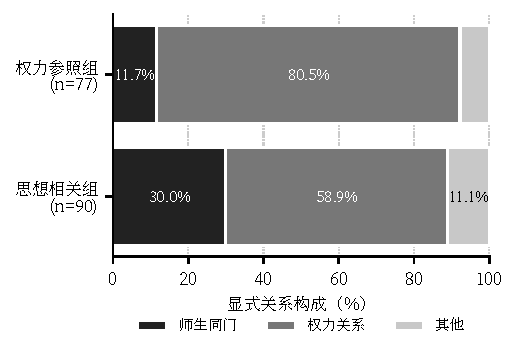
\includegraphics[width=\columnwidth]{figures/fig_ideology_1.pdf}
\caption{思想相关组与权力参照组的显式关系构成。思想组的师生同门占比更高，但权力关系仍占过半；类别为互斥编码。}
\label{fig:ideology-composition}
\end{figure}

全图“师生同门”只有63条，占2.7\%；但在10名思想相关人物的90条显式关系中，该类有27条、占30.0\%，高出全图基线。权力参照组有77条显式关系，其中师生同门9条、占11.7\%。恢复自动推导边后，两组相应占比降为18.2\%与7.3\%，方向不变。由此可见，师承确是思想人物的区别性连接方式，而不是全图普遍现象。

但“区别性”不等于“自治”。思想组的君臣从属、政治攻讦、敌对冲突、同盟友党合计53条，占58.9\%，仍高于师承边；参照组为62条，占80.5\%。思想传播网络并非悬浮在朝廷之外，而是以较高的师承比例嵌入一个仍由权力关系占多数的网络。图\ref{fig:ideology-composition}因此不支持“思想先自由生长、随后才被权力碰触”的简单二阶段模型。

\begin{table}[!t]
\caption{六个锚点的显式关系构成}
\label{tab:ideology-anchors}
\centering
\begin{tabular}{@{}lrrrr@{}}
\toprule
人物 & 度数 & 显式边 & 师生同门 & 权力关系 \\
\midrule
王守仁 & 50 & 36 & 8（22.2\%） & 21（58.3\%）\\
徐阶 & 67 & 42 & 17（40.5\%） & 24（57.1\%）\\
顾宪成 & 18 & 7 & 1（14.3\%） & 4（57.1\%）\\
高攀龙 & 11 & 1 & 1（100.0\%） & 0（0.0\%）\\
张居正 & 66 & 45 & 8（17.8\%） & 35（77.8\%）\\
严嵩 & 59 & 33 & 1（3.0\%） & 28（84.8\%）\\
\bottomrule
\end{tabular}
\end{table}

锚点差异进一步阻止我们把“思想型”本质化。王守仁度数50，显式边中师生同门与政治攻讦各8条；徐阶度数67，17条师生同门使其传播占比达到40.5\%，但其24条权力关系仍占57.1\%。张居正度数66，师生同门也有8条，说明权力人物同样通过门生网络运作。真正形成对照的是严嵩：33条显式边中敌对冲突14条、政治攻讦7条，而师生同门仅1条。可计算的结论不是“思想人物没有权力”，而是思想相关人物把师承通道带进了权力网络。

\subsection{时间序列：形成、间隔与制度冲突}

\begin{figure}[!t]
\centering
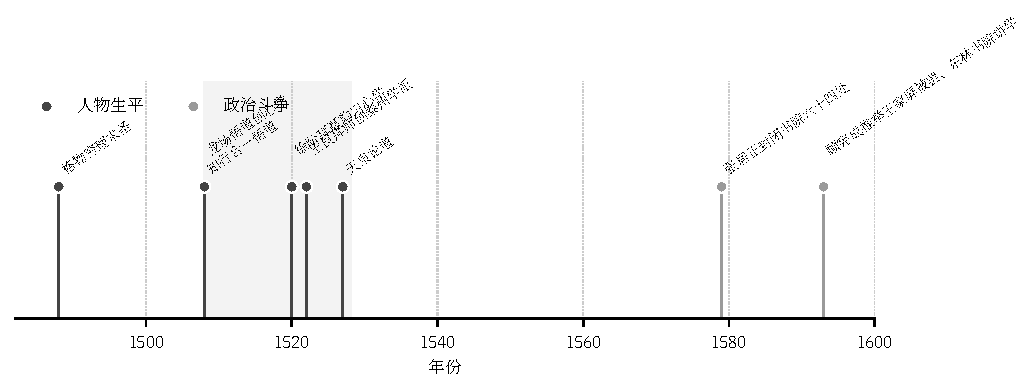
\includegraphics[width=\columnwidth]{figures/fig_ideology_2.pdf}
\caption{8件思想相关事件的年份分布。1508--1528窗口集中5件形成与传播事件，1579与1593出现两件被编码为政治斗争的书院事件。}
\label{fig:ideology-timeline}
\end{figure}

8件事件中，1488年“格物穷理”构成前史；1508年同时出现“龙场悟道创心学”和“知行合一悟道”；1520年徐阶拜聂豹习心学，1522年王艮拜师创泰州学派，1527年天泉论道。因而1508--1528窗口集中了5件，占全部8件的62.5\%。1529--1578窗口没有符合窄筛选规则的事件，这一空白只能解释为本书编码的叙事间隔，不能解释为思想活动中止。

晚期两个节点改变了类别。原书逐字写“万历七年（1579），张居正下令，关闭天下书院，共计六十四处”；结构化事件将其编码为政治斗争。1593年的顾宪成罢官与东林书院讲学同样被编码为政治斗争。8件思想事件中，人物生平6件、占75.0\%，政治斗争2件、占25.0\%。从形成到制度冲突的转折真实存在于叙事编码中，但“收编”不是直接字段：关闭书院、讲学入党争只是可观察替代量。

\subsection{反例与边界情形}

高攀龙显式关系仅1条，恰为师生同门，导致100.0\%这一比例极不稳定；顾宪成显式关系7条且七类各1条，同样不宜单独外推。另一方面，何心隐到王守仁的再传弟子关系被编码为“亲属”，暴露类别噪声。组层面的90条显式边比单人百分比稳健，但仍受抽取规则约束。本文因此把个体表作为诊断，不把它当作精确人物排名。

\section{讨论与限制}

\subsection{“突围/收编”的可测边界}

结果支持一种比标题更克制的解释：思想相关人物在关系图中确有较高比例的师承边，但他们的大多数显式关系仍通向朝廷权力。所谓“突围”可由师生同门占比和1508--1528年的传播事件簇近似；所谓“收编”只能由权力关系占比、1579年关闭书院和1593年讲学入党争近似。两者都是分析者施加的框架，不是数据直接吐出的标签。本文不声称测得思想自由度，也不把书院关闭与所有思想控制画等号。

\subsection{首要效度威胁：没有思想文本本身}

本文最大的限制不是样本量，而是材料性质。语料只有通俗史著中的叙事提及，没有《传习录》原文、门人问答、书院规约、奏疏或讲会记录。于是“知行合一”12次只表示这个字符串在叙事中出现12次，不能说明命题被讨论了12次，更不能衡量读者接受。叙事作者把王守仁写成能平叛的行动者，也会同时提高其政治事件数与关系度数；这种写法本身就是研究对象，却使思想内容与叙事情节无法分离。

\subsection{关系抽取与分组内造}

关系类别由项目抽取体系预先定义。“师生同门”把严格师承、同门、门生与思想认同放在一类；四类“权力关系”则同时包含制度隶属、攻讦、冲突与联盟。它们适合做结构描述，不适合推断情感或动机。思想组名单也由同一语料的角色、事件与关系标记确定，存在同源自证。剔除58条思想组推导边后，师承占比从18.2\%升到30.0\%，说明自动共现对构成有显著影响；但稳健性方向未翻转。

\subsection{外推与复现}

本研究只是一部书、一个抽取版本的案例。要讨论明代思想传播本身，下一步至少应加入思想原典与不同史著，区分著述、讲会、科举、官僚任迁四种关系，并让不同标注者独立复核类别。本文公开统计底稿、筛选规则与两份作图脚本；版权文本不公开，但每处书内证据都保留逐字命中次数。引用只使用核验通过的条目，语料书籍按无 DOI 版本信息列示。

\section{结论}

本文没有把“心学突围、朝廷收编”当成一个已测得的历史事实，而是把它拆成关系构成与时间序列：思想相关组的显式关系中，师生同门占30.0\%，权力关系占58.9\%，显示传播与权力接合同时发生。

时间线上，1508--1528年集中了形成与传授事件，1579与1593年的书院节点进入政治斗争类别；这支持“叙事从个人悟道转向制度冲突”的语料内判断。

可检验的下一步，是把原典、奏疏和书院档案加入独立语料，重标关系类别并比较同一批人物。若组间构成和时间转折仍然出现，解释框架才有资格越过这一本通俗史著。


\bibliographystyle{IEEEtran}
\bibliography{references}

\end{document}
